\documentclass[tikz]{standalone}
\usetikzlibrary{arrows.meta, positioning}
\begin{document}
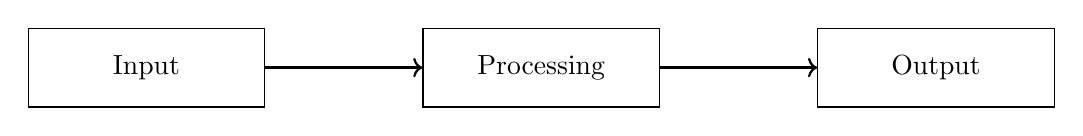
\begin{tikzpicture}[
  box/.style={draw, rectangle, minimum width=3cm, minimum height=1cm},
  arrow/.style={->, thick}
]
  \node[box] (a) {Input};
  \node[box, right=2cm of a] (b) {Processing};
  \node[box, right=2cm of b] (c) {Output};

  \draw[arrow] (a) -- (b);
  \draw[arrow] (b) -- (c);
\end{tikzpicture}
\end{document}
